\subsection{Primitive relative spectral dynamics}

The carrier theorem is not intended to float above an unspecified microscopic dynamics.
The starting point is therefore the admissible reduced datum from which the primitive layer is
reconstructed before the later closure theorems are invoked.

\begin{definition}[Admissible reduced theorem datum]
\label{def:reduced-theorem-datum}
The admissible reduced datum is
\[
\Tmin^{\mathrm{adm}}:=(\mathcal A,\mathcal H,D,J,\Gamma,\inv,\nu)
\]
with the following built-in admissibility conditions:
\begin{enumerate}[label=(\roman*), leftmargin=1.5em, topsep=3pt, itemsep=2pt]
    \item $Z(\mathcal A)$ is spectrally regular and its Gelfand spectrum is a smooth compact oriented manifold $\widetilde M$;
    \item $\inv$ acts by a smooth order-two involution on $Z(\mathcal A)$, commutes with $J$ and $\Gamma$, and has smooth fixed locus $\Seam:=\mathrm{Fix}(\inv)$;
    \item in a collar neighborhood of $\Seam$, the Dirac operator has canonical product form
    \[
    D=\gamma_n(\partial_n+B_\Sigma);
    \]
    \item the cutoff profile is generated by a positive complete-Bernstein measure
    \begin{equation}
    \label{eq:bernstein-test-function}
    f(x)=\int_0^\infty e^{-t x^2}\,d\nu(t),
    \qquad
    d\nu(t)\ge 0;
    \end{equation}
    \item the seam collar is reflection-regular so that the doubled operator and admissibility complex defined later are well posed on the same datum.
\end{enumerate}
\end{definition}

\begin{assumption}[Almost commutative factorization of the Hilbert space]
\label{ass:almost-commutative-factorization}
The reduced datum admits an almost commutative factorization
\[
\mathcal H\cong L^2(\widetilde M,S)\otimes \Hint,
\]
with $S\to\widetilde M$ the spinor bundle on the oriented double cover and $\Hint$ a finite
internal Hilbert space.
\end{assumption}

\begin{theorem}[Primitive kinematic scaffold reconstructed from the admissible reduced datum]
\label{thm:primitive-datum-from-reduced-datum}
\label{thm:primitive-scaffold-from-reduced-datum}
Let $\Tmin^{\mathrm{adm}}$ be as above. Then the primitive kinematic scaffold is reconstructed
canonically as
\[
\widetilde M=\mathrm{Spec}\,Z(\mathcal A),\qquad
M=\widetilde M/\inv,\qquad
\Seam=\mathrm{Fix}(\inv),\qquad
X=\widetilde M\setminus \Seam,
\]
\[
D_{\mathrm{ref}}:=\frac12(D+\inv D\inv),\qquad
D_{\mathrm{rel}}:=\frac12(D-\inv D\inv),\qquad
\chiseed:=\lambda_1^+(|B_\Sigma|)^{-1}.
\]
Hence the primitive scaffold
\[
\Tprim^{\mathrm{kin}}
:=
(X,\widetilde M,M,\Seam,\inv,D_{\mathrm{ref}},D_{\mathrm{rel}},f,\chiseed)
\]
is derived, not assumed.
If one further chooses an almost-commutative factorization
\[
\mathcal H_{\mathrm{prim}}\cong L^2(X,S)\otimes \Hint,
\]
then $S$ and $\Hint$ refer to that chosen factorization and are not claimed as
additional reconstruction outputs of the present theorem.
\end{theorem}

\begin{corollary}[No residual primitive topology or comparison-operator ontology]
Within TFPT the oriented double cover, the physical quotient, the seam, the
reference/relative operator pair, and the primitive seam response are theorem-level outputs of
$\Tmin^{\mathrm{adm}}$. Under \Cref{ass:almost-commutative-factorization}, no additional
primitive topology or comparison-operator ontology remains in the main-text scaffold.
\end{corollary}

\begin{definition}[Primitive Euclidean action]
The primitive Euclidean action is the relative spectral seed
\[
S_{\mathrm{prim}}[\chiseed]
:=
\tr f\!\left(\frac{D_{\mathrm{rel}}}{\chiseed}\right)
-
\tr f\!\left(\frac{D_{\mathrm{ref}}}{\chiseed}\right)
+\frac{i\pi}{2}\Delta\eta_\Sigma.
\]
Gauge fixing, ghosts, carrier-compatible bosonic fluctuations, and the admissibly compressed net
\[
\mathfrak A_{\mathrm{adm}}(\mathcal O):=
\Padm\,\mathfrak A(\mathcal O)\,\Padm.
\]
are introduced only after the hard carrier theorem and the later admissibility closure package are in place.
\end{definition}

\begin{theorem}[Bernstein superposition on a positive branch]
\label{ass:bernstein-positivity}
Assume that for every $t>0$ the heat semigroup
\[
e^{-tD_{\mathrm{geo}}^2/\chiseed^2}
\]
is positivity preserving and reflection stable on the seam-even bosonic branch.
If
\[
f(z)=\int_0^\infty e^{-tz^2}\,d\nu(t),\qquad d\nu(t)\ge 0,
\]
then the corresponding Bernstein superposition inherits positivity and reflection stability.
\end{theorem}

\begin{proof}[Proof sketch]
Each heat kernel $e^{-tD_{\mathrm{geo}}^2/\chiseed^2}$ is positivity preserving and reflection
stable on the seam-even bosonic branch by assumption. Positive superposition with
$d\nu(t)\ge 0$ preserves both properties, so the Bernstein profile inherits them immediately.
\end{proof}

\begin{theorem}[Well-posed primitive dynamics]
Assume the geometric anchor admits a self-adjoint Fredholm APS realization on the declared
domain $\APSdom$, and $D_{\mathrm{rel}}$ is relatively bounded with respect to that realization.
Then the finite-cutoff relative spectral seed is well defined before carrier and admissibility
closure are imposed.
\end{theorem}

\begin{proof}[Proof sketch]
Dirac-type operators with APS boundary data admit self-adjoint Fredholm realizations on the
corresponding Sobolev graph domain. Since $D_{\mathrm{rel}}$ is relatively bounded with respect
to the geometric anchor, both operators share the same graph domain and the relative spectral
seed is well defined at every finite cutoff.
\end{proof}

\begin{remark}[APS roles on the admissible branch]
$\APSdom$ is the primitive elliptic boundary choice for the geometric anchor. The family
pairing structure is induced later on the doubled admissible branch and is therefore not a
second primitive input package.
\end{remark}

\begin{figure}[t]
\centering
\scriptsize
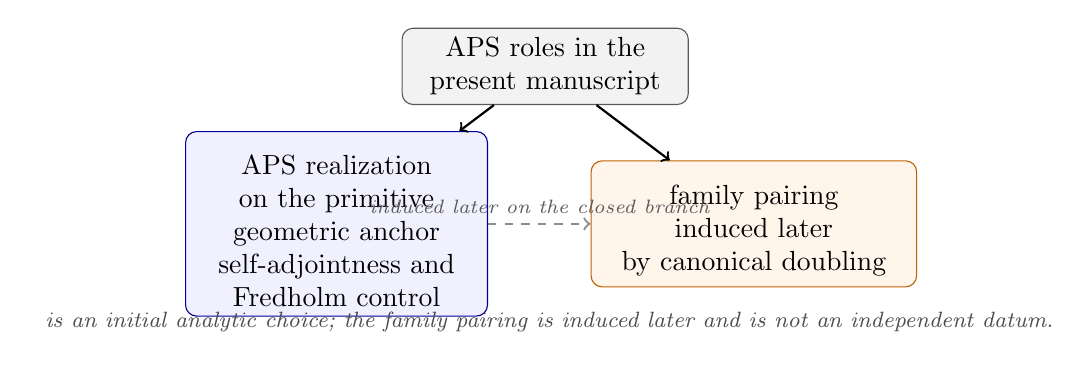
\begin{tikzpicture}[
    root/.style={draw=black!65, fill=gray!10, rounded corners, text width=3.4cm, minimum height=0.9cm, align=center},
    dom/.style={draw=blue!60!black, fill=blue!6, rounded corners, text width=3.6cm, minimum height=1.6cm, align=center},
    fam/.style={draw=orange!75!black, fill=orange!8, rounded corners, text width=3.9cm, minimum height=1.6cm, align=center},
    note/.style={font=\footnotesize\itshape, text=black!70, align=center}
]
\node[root] (aps) at (0,0) {APS roles in the present manuscript};
\node[dom] (dom) at (-2.65,-2.0) {\textbf{$\APSdom$}\\APS realization on the primitive geometric anchor\\self-adjointness and Fredholm control};
\node[fam] (fam) at (2.65,-2.0) {\textbf{$\APSfam$}\\family pairing induced later\\by canonical doubling};
\draw[->, thick] (aps) -- (dom);
\draw[->, thick] (aps) -- (fam);
\draw[->, dashed, black!45, line width=0.8pt] (dom.east) -- node[above, sloped, font=\scriptsize\itshape, text=black!65] {induced later on the closed branch} (fam.west);
\node[note] at (0,-3.25) {$\APSdom$ is an initial analytic choice; the family pairing is induced later and is not an independent datum.};
\end{tikzpicture}
\caption{APS organization in the present draft. $\APSdom$ is the primitive elliptic boundary
choice. The family pairing structure is induced later on the doubled admissible branch and is
therefore not a second primitive input package.}
\label{fig:aps-split}
\end{figure}

\begin{corollary}[Carrier-compatible Lorentzian dynamics after closure]
Once the later carrier-compatible fluctuation package and the admissibility closure hypotheses of \Cref{sec:closure-theorems} are imposed, the resulting admissible Euclidean theory reconstructs a self-adjoint Lorentzian Hamiltonian $H_{\mathrm{adm}}$ and a one-parameter automorphism group
\[
\alpha_t(O)=e^{itH_{\mathrm{adm}}}Oe^{-itH_{\mathrm{adm}}}.
\]
\end{corollary}

\subsection{Minimal carrier theorem}
\label{sec:minimal-carrier-proof}

\begin{theorem}[Minimal carrier theorem]
Let $E=E_b\oplus E_s$ be a split carrier with traceless diagonal generator
\[
Y_{b,s}
=
\mathrm{diag}\!\left(
\underbrace{-\frac1b,\ldots,-\frac1b}_{b\ \text{times}},
\underbrace{\frac1s,\ldots,\frac1s}_{s\ \text{times}}
\right).
\]
If one simultaneously requires
\begin{equation}
\label{eq:minimal-carrier-conditions}
\dim \Lambda^{\mathrm{even}}E=16,
\qquad
\tr_E Y_{b,s}^2=\frac56,
\end{equation}
then necessarily $\{b,s\}=\{3,2\}$.
\end{theorem}

\begin{proof}
Write $g=b+s$. Since
\[
\dim \Lambda^{\mathrm{even}}E=2^{g-1},
\]
the first condition gives $g=5$. For the diagonal generator above one has
\[
\tr_E Y_{b,s}^2
=
b\left(\frac{1}{b^2}\right)+s\left(\frac{1}{s^2}\right)
=
\frac1b+\frac1s
=
\frac{b+s}{bs}
=
\frac{5}{bs}.
\]
Imposing $\tr_E Y_{b,s}^2=5/6$ yields $bs=6$. Together with $b+s=5$ this forces the unordered solution $\{b,s\}=\{3,2\}$.
\end{proof}

Hence from now on
\[
E=E_3\oplus E_2,
\qquad
P_3=\frac{\mathbf 1-\inv}{2},
\qquad
P_2=\frac{\mathbf 1+\inv}{2},
\]
and the hypercharge operator is read concretely as
\begin{equation}
\label{eq:explicit-hypercharge}
Y
=
\mathrm{diag}\!\left(-\frac13,-\frac13,-\frac13,\frac12,\frac12\right)
=
-\frac13 P_3+\frac12 P_2
=
\frac1{12}\mathbf 1+\frac5{12}\inv.
\end{equation}

\begin{lemma}[Hypercharge--seam inversion]
On the minimal carrier, the seam involution is recovered from hypercharge by
\begin{align}
\inv&=\frac{12Y-\mathbf 1}{5},
\label{eq:hypercharge-seam-inversion}\\
(12Y-\mathbf 1)^2&=25\,\mathbf 1,
\nonumber\\
6Y^2-Y-\mathbf 1&=0.
\label{eq:carrier-polynomial}
\end{align}
Consequently the carrier projectors are
\[
P_2=\frac{\mathbf 1+\inv}{2}=\frac{2(3Y+\mathbf 1)}{5},
\qquad
P_3=\frac{\mathbf 1-\inv}{2}=\frac{3(\mathbf 1-2Y)}{5}.
\]
\end{lemma}

\begin{proof}
The affine relation between $Y$ and $\inv$ is inverted algebraically. Squaring the result and using $\inv^2=\mathbf 1$ gives the quadratic carrier polynomial. The projector formulas then follow from $P_2=(\mathbf 1+\inv)/2$ and $P_3=(\mathbf 1-\inv)/2$.
\end{proof}

The hard carrier package is summarized visually in \Cref{fig:minimal-carrier-glance}. The point is that the same minimal data are readable in two equivalent ways: geometrically as an oriented double cover with seam involution, and algebraically as the $3+2$ carrier split with two spectral hypercharges.

\begin{figure}[t]
\centering
\footnotesize
\begin{tikzpicture}[
    >=Latex,
    slot3/.style={draw=blue!60!black, fill=blue!6, rounded corners, minimum width=0.72cm, minimum height=0.72cm, align=center},
    slot2/.style={draw=orange!70!black, fill=orange!9, rounded corners, minimum width=0.72cm, minimum height=0.72cm, align=center},
    info/.style={draw=black!55, rounded corners, fill=gray!3, align=center, inner sep=5pt}
]
\node[font=\bfseries] at (-3.5,1.95) {oriented double cover};
\draw[draw=gray!70!black, fill=gray!6, rounded corners] (-5.4,0.55) rectangle (-1.7,1.35);
\draw[draw=gray!70!black, fill=gray!6, rounded corners] (-5.4,-1.35) rectangle (-1.7,-0.55);
\node at (-3.55,0.95) {upper sheet};
\node at (-3.55,-0.95) {lower sheet};
\draw[very thick, purple!70!black] (-5.6,0) -- (-1.45,0);
\node[anchor=west, purple!70!black] at (-1.38,0) {seam $\Sigma$};
\draw[<->, thick] (-3.55,0.42) -- (-3.55,-0.42);
\node[anchor=west] at (-3.4,0) {$\iota$};

\node[font=\bfseries] at (2.35,1.95) {minimal carrier split};
\node[slot3] (c1) at (0.55,0.95) {$c_1$};
\node[slot3, right=2mm of c1] (c2) {$c_2$};
\node[slot3, right=2mm of c2] (c3) {$c_3$};
\node[slot2, right=6mm of c3] (w1) {$w_1$};
\node[slot2, right=2mm of w1] (w2) {$w_2$};
\node[align=center, blue!60!black] at ($(c2.south)+(0,-0.45)$) {$E_3=P_3E$\\three color slots};
\node[align=center, orange!75!black] at ($(w1.south)+(0.45,-0.45)$) {$E_2=P_2E$\\two weak slots};
\draw[decorate, decoration={brace, amplitude=4pt}] ($(c1.north west)+(-0.07,0.12)$) -- ($(c3.north east)+(0.07,0.12)$);
\node[blue!60!black] at ($(c2.north)+(0,0.42)$) {$3$};
\draw[decorate, decoration={brace, amplitude=4pt}] ($(w1.north west)+(-0.07,0.12)$) -- ($(w2.north east)+(0.07,0.12)$);
\node[orange!75!black] at ($(w1.north east)+(0.2,0.42)$) {$2$};

\node[info] at (-0.45,-2.3) {%
    $\displaystyle
    Y=-\frac13 P_3+\frac12 P_2
    =\frac1{12}\mathbf 1+\frac5{12}\iota
    \qquad
    \iota=\frac{12Y-\mathbf 1}{5}
    $\\[2pt]
    $\displaystyle
    P_3=\frac{\mathbf 1-\iota}{2},
    \qquad
    P_2=\frac{\mathbf 1+\iota}{2},
    \qquad
    \mathrm{Spec}(Y)=\left\{-\frac13,\frac12\right\}
    $};
\end{tikzpicture}
\caption{Minimal carrier at a glance. The seam involution and the hypercharge operator carry the same hard two-point information: geometrically they separate the two sheets, and algebraically they separate the $3+2$ carrier split through the projectors $P_3$ and $P_2$.}
\label{fig:minimal-carrier-glance}
\end{figure}

\begin{remark}[Two-point carrier algebra]
Because the minimal carrier satisfies $6Y^2-Y-\mathbf 1=0$, every analytic function of $Y$ reduces to
\[
f(Y)=A_f\,\mathbf 1+B_f\,Y,
\qquad
A_f=\frac{2f(1/2)+3f(-1/3)}{5},
\qquad
B_f=\frac{6\bigl(f(1/2)-f(-1/3)\bigr)}{5}.
\]
Thus the hard carrier is effectively a two-point algebra supported on the spectral values $-1/3$ and $1/2$, and the projectors $P_3,P_2$ are already polynomial functions of $Y$.
\end{remark}

\begin{remark}[Factorized carrier polynomial and carrier discriminant]\label{rem:carrier-discriminant}
For a general split carrier $E=E_b\oplus E_s$ with total rank $g:=b+s$ and eigenvalues $-1/b$ and $1/s$, the carrier generator satisfies
\[
\left(Y+\frac{1}{b}\right)\left(Y-\frac{1}{s}\right)=0
\quad\Longleftrightarrow\quad
bs\,Y^2+(s-b)Y-\mathbf 1=0.
\]
Its discriminant is
\[
\Delta_Y=(s-b)^2+4bs=(b+s)^2=g^2.
\]
Thus the square root of the carrier discriminant is the carrier rank itself. Moreover,
\[
Y=\frac{b-s}{2bs}\,\mathbf 1+\frac{g}{2bs}\,\inv,
\qquad
\inv=\frac{2bs\,Y-(b-s)\,\mathbf 1}{g}.
\]
On the minimal branch $(b,s)=(3,2)$, this reduces to
\[
6Y^2-Y-\mathbf 1=(2Y-\mathbf 1)(3Y+\mathbf 1),
\qquad
\Delta_Y=25=5^2,
\qquad
\inv=\frac{12Y-\mathbf 1}{5}.
\]
Hence the denominator $5$ in the hypercharge--seam inversion is exactly $\sqrt{\Delta_Y}$, not an additional inserted constant.

This does not replace the stabilizer proof of
\[
G_{\SM}^{\mathrm{glob}}=S(U(3)\times U(2)),
\]
which is the actual source of the global Standard Model quotient in the present manuscript. What the factorization and discriminant do show exactly is that the hard carrier already supports the distinguished spectral values
\[
Y=\frac{1}{2},
\qquad
Y=-\frac{1}{3},
\]
and that the inversion denominator is fixed algebraically by the carrier discriminant.
\end{remark}

The two carrier invariants used repeatedly below are
\[
\gamma=\tr_EY^2=\frac56,
\qquad
B=\frac{\rank E_3}{\rank E_2}=\frac32.
\]
\begin{corollary}[Carrier norm from the carrier polynomial]
The carrier polynomial already fixes
\[
\gamma=\tr_EY^2=\frac16\tr_E(Y+\mathbf 1)=\frac56,
\]
since $\tr_EY=0$ and $\rank E=5$.
\end{corollary}

\begin{corollary}[Minimal carrier compression]
\label{cor:minimal-carrier-compression}
On the minimal carrier branch,
\[
B\gamma=\frac32\cdot\frac56=\frac54.
\]
\end{corollary}

We package the hard kernel as
\[
\Cmin=(E_3\oplus E_2,\ Y,\ S^+,\ \gamma,\ B).
\]

